\documentclass{article}
\usepackage[dvipdfmx]{graphicx}
\usepackage{here}
\usepackage{amsmath}
\usepackage{amsfonts}
\usepackage{cite}
\allowdisplaybreaks[1]

\title{README for the scripts in ionizer45}
\author{N. Ozawa}
\date{\today}

\begin{document}
\maketitle

\section{Prerequisites}
The scripts are to be used with the beam simulation program SIMION or any program of that sort that could generate a data file containing the trajectory point of each timestep for all the particles in the following form:
\begin{table}[H]
  \begin{tabular}{lccc}
    Ion no. & X & Y & Z \\
    1 & $x_{11}$ & $y_{11}$ & $z_{11}$ \\
    1 & $x_{12}$ & $y_{12}$ & $z_{12}$ \\
    1 & $x_{13}$ & $y_{13}$ & $z_{13}$ \\
    $\cdots$ & $\cdots$ & $\cdots$ & $\cdots$ \\
    2 & $x_{21}$ & $y_{21}$ & $z_{21}$ \\
    $\cdots$ & $\cdots$ & $\cdots$ & $\cdots$
  \end{tabular}
\end{table}
The data will be in the coordinates used in the simulation program, which could differ from the coordinates used in Autodesk Inventor. For SIMION, the directions of the $x$, $y$, and $z$ axes are the same, but the origin differs. It is assumed that the vertical axis (i.e. the primary beam axis) is the $z$ axis, and the extraction axis is tilted 45 degrees towards the $x$ axis i.e. $z_{{\rm Inventor}} = x_{{\rm Inventor}}$ and $y_{{\rm Inventor}} = 0$. \\

In this document, the subscript $I$ denotes Inventor coordinates and the subscript $S$ denotes the SIMION coordinates.


\section{trajectory\_display.cpp}
This script obtains all the trajectory points from the data file and plots them in Inventor Coordinates. For simplicity, one graph projects the trajectories in the $z_I$-$x_I$ plane, and the other in the $x_I$-$y_I$ plane. Additionally, it fits the trajectory points with the function $z_I = ax_I + b$ with $a$ and $b$ as free parameters. This will check the extraction direction of the Fr beam. Ideally, $a$ should be close to 1 and $b$ should be close to 0. The term "gradient" is used for $a$ and it is an important parameter for the geometry optimization of the plate electrode.




\section{bpm45.cpp}
This script displays the 2D histogram of the beam profile. The beam profile is taken at an imaginary monitor tilted 45 degrees from the $y_I-z_I$ plane with respect to the $y_I$ axis and shifted distance $w$ away from the origin $(0,0,0)_I$. This imaginary monitor can be mathematically described as the set 
\begin{equation*}
P(w) = \left\{ (x,y,z)_I | z_I = -x_I + \sqrt{2}w, y_I \in \mathbb{R} \right\}.
\end{equation*}
For an ideal extraction, the Fr ion beam trajectory is exactly equivalent to the line $z_I = x_I$, which yields a beam profile of a single point
\begin{equation*}
\vec{BPM}(w) = \left(
\begin{array}{c}
	\frac{w}{\sqrt{2}}\\
	0 \\
	\frac{w}{\sqrt{2}}
\end{array} \right)_I.
\end{equation*}
However, for the actual beam, each ion has a trajectory point
\begin{equation*}
\vec{trj}(w) = \left(
\begin{array}{c}
	trjptx \\
	trjpty \\
	trjptz
\end{array} \right)_I
\end{equation*}
where the ion hits the imaginary monitor $P(w)$. Here we can define a new coordinate $P$, which is the coordinate on the surface of the imaginary monitor. This can be obtained by taking the difference of any point in Inventor coordinates with $\vec{BPM}$. Thus, 
\begin{equation*}
\vec{trj}(w) = \left(
\begin{array}{c}
	trjptx - \frac{w}{\sqrt{2}} \\
	trjpty \\
	trjptz - \frac{w}{\sqrt{2}}
\end{array} \right)_P . \\
\end{equation*}

Furthurmore, we can define a coordinate $M$ which is the coordinate system that corresponds to the $x_M$-$y_M$ plane defined on the MCP screen. This can be understood as the "observed" coordinate system as if the imaginary monitor is examined from the downstream side of the beamline. By plotting the 2D histogram of the $\vec{trj}$ points in the $M$ coordinates, we obtain the actual image obtained behind the MCP and Phosphor screen. For example, a trajectory that is shifted upwards from the ideal extraction line will appear as a trajectory point shifted in the positive $y_M$ direction, and a trajectory that is shifted right from the ideal extraction line will appear as a trajectory point shifted in the negative $x_M$ direction. \\

From the definition of $P(w)$, we can shift from the $P$ coordinates to the $M$ coordinates by first rotating 45 degrees around the $y_I$ axis
\begin{equation*}
R_y = \frac{1}{\sqrt{2}} \left(
\begin{array}{ccc}
	1 & 0 & -1 \\
	0 & \sqrt{2} & 0 \\
	1 & 0 & 1
\end{array} \right)
\end{equation*}
and then rotating -90 degrees around the $z_I$ axis
\begin{equation*}
R_z = \left(
\begin{array}{ccc}
	0 & 1 & 0 \\
	-1 & 0 & 0 \\
	0 & 0 & 1
\end{array} \right).
\end{equation*}
The first and second components yield the $x_M$ and $y_M$ coordinate values of the trajectory point, and the third component corresponds to the distance of the trajectory point to the monitor $P(w)$. Especially, when this third component is positive, the trajectory has already passed across $P(w)$, and when it is negative, the trajectory has not yet reached $P(w)$. \\

Now we establish the method of calculating the trajectory point in $M$ coordinates based on the simulation data. First, by collecting the starting points of the trajectories, we obtain the origin of the Inventor coordinates in SIMION coordinates
\begin{equation*}
\vec{v_{SI}} = \left(
\begin{array}{c}
	x_{SI} \\
	y_{SI} \\
	z_{SI} + h
\end{array} \right)
\end{equation*}
where $h$ is the distance of the Au target below the origin. The $x_{SI}$ and $y_{SI}$ values can be obtained by taking the average values of all the ions. By using these values any points stored in the data file could be converted to Inventor coordinates. \\

\begin{figure}[H]
  \begin{center}
    \includegraphics[width=10.0cm]{./bpm45_fig.png}
    \caption{The method of obtaining the beam profile.}
    \label{fig:bpm45_fig}
  \end{center}
\end{figure}

Only discrete points are recorded in the data file, so usually the trajectory point will be between the point $\vec{P_f}$ right after $P(w)$ and the point $\vec{P_b}$ right before $P(w)$. These points could be searched for in the following way:
\begin{enumerate}
	\item Pick a trajectory point $\vec{P}$ in the data file.
	\item Record the $\vec{P}$ as the "previous point" $\vec{P_2}$ and define the succeeding point as the "next point" $\vec{P_1}$.
	\item Step forward one point at a time and calculate the third component of $\vec{P_1}$ in $M$ coordinates.
	\item When the third component of $\vec{P_1}$ in $M$ coordinates becomes non-negative, define $\vec{P_f} = \vec{P_1}$ and $\vec{P_b} = \vec{P_2}$.
\end{enumerate}
The components could be written explicitly as
\begin{eqnarray*}
\vec{P_f} & = & \left(
\begin{array}{c}
	x_{sf} \\
	y_{sf} \\
	z_{sf}
\end{array} \right)_S = \left(
\begin{array}{c}
	x_{sf} - x_{SI} \\
	y_{sf} - y_{SI} \\
	z_{sf} - z_{SI} - h
\end{array} \right)_I \\
\vec{P_b} & = & \left(
\begin{array}{c}
	x_{sb} \\
	y_{sb} \\
	z_{sb}
\end{array} \right)_S = \left(
\begin{array}{c}
	x_{sb} - x_{SI} \\
	y_{sb} - y_{SI} \\
	z_{sb} - z_{SI} - h
\end{array} \right)_I
\end{eqnarray*}
in each coordinate system. In the script, the third component of $\vec{P_f}$ in $M$ coordinates is calculated by
\begin{eqnarray*}
& & \left( 
\begin{array}{ccc}
	0 & 0 & 1
\end{array} \right) R_z R_y \left( \vec{P_f}_I - \vec{BPM}(w) \right) \\
& = & \frac{1}{\sqrt{2}} \left(
\begin{array}{ccc}
	0 & 0 & 1
\end{array} \right) \left(
\begin{array}{ccc}
	0 & 1 & 0 \\
	-1 & 0 & 0 \\
	0 & 0 & 1
\end{array} \right) \left(
\begin{array}{ccc}
	1 & 0 & -1 \\
	0 & \sqrt{2} & 0 \\
	1 & 0 & 1
\end{array} \right) \left(
\begin{array}{c}
	x_{sf} - x_{SI} - \frac{w}{\sqrt{2}} \\
	y_{sf} - y_{SI} \\
	z_{sf} - z_{SI} - h - \frac{w}{\sqrt{2}}
\end{array} \right)_P \\
& = & \frac{1}{\sqrt{2}} \left(
\begin{array}{ccc}
	1 & 0 & 1
\end{array} \right) \left(
\begin{array}{c}
	x_{sf} - x_{SI} - \frac{w}{\sqrt{2}} \\
	y_{sf} - y_{SI} \\
	z_{sf} - z_{SI} - h - \frac{w}{\sqrt{2}}
\end{array} \right)_P \\
& = & \frac{x_{sf}-x_{SI}+z_{sf}-z_{SI}-h}{\sqrt{2}} - w. \\
\end{eqnarray*}

In order to find the trajectory point on $P(w)$, we assume that the ion flies in a straight line from point $\vec{P_b}$ to point $\vec{P_f}$. Then, using a parameter $t_{trj}(w)$ such that $0 \le t_{trj}(w) < 1$, and rewriting the two points as
\begin{eqnarray*}
\vec{d} & = & \vec{P_f} - \vec{P_b} \\
& = & \left(
\begin{array}{c}
	x_{sf} - x_{sb} \\
	y_{sf} - y_{sb} \\
	z_{sf} - z_{sb}
\end{array} \right) =: \left(
\begin{array}{c}
	x_d \\
	y_d \\
	z_d
\end{array} \right) \\
\vec{P_b} & = & \left(
\begin{array}{c}
	x_{sb} - x_{SI} \\
	y_{sb} - y_{SI} \\
	z_{sb} - z_{SI} - h
\end{array} \right)_I =: \left(
\begin{array}{c}
	x_0 \\
	y_0 \\
	z_0
\end{array} \right),
\end{eqnarray*}
the trajectory point on $P(w)$ can be identified by
\begin{equation*}
\vec{trj}(w) = t_{trj}(w) \vec{d} + \vec{P_b} = \left(
\begin{array}{c}
	t_{trj} x_d + x_0 \\
	t_{trj} y_d + y_0 \\
	t_{trj} z_d + z_0
\end{array} \right).
\end{equation*}
Recalling the definition of $P(w)$, the condition for the trajectory point to be on the plane $P(w)$ is $trjptz = -trjptx + \sqrt{2}w$, thus
\begin{eqnarray*}
t_{trj} z_d + z_0 & = & -t_{trj} x_d - x_0 + \sqrt{2}w \\
t_{trj} (z_d + x_d) & = & -z_0 - x_0 + \sqrt{2}w \\
t_{trj} & = & \frac{-z_0-x_0+\sqrt{2}w}{z_d+x_d}. \\
\end{eqnarray*}

Therefore, after the points $\vec{P_f} = \left(
\begin{array}{c}
	x_d + x_0 \\
	y_d + y_0 \\
	z_d + z_0
\end{array} \right)_I$ and $\vec{P_b} = \left(
\begin{array}{c}
	x_0 \\
	y_0 \\
	z_0
\end{array} \right)_I$ have been determined from the data file and the parameter $t_{trj}(w) = \frac{-z_0-x_0+\sqrt{2}w}{z_d+x_d}$ has been calculated, the trajectory point on $P(w)$ in $M$ coordinates is estimated by
\begin{eqnarray*}
\vec{trj}(w)_M & = & R_z R_y \left\{ t_{trj}(w) \left( \vec{P_f}_I - \vec{P_b}_I \right) + \vec{P_b}_I - \vec{BPM}(w) \right\} \\
& = & \frac{1}{\sqrt{2}} \left(
\begin{array}{ccc}
	0 & 1 & 0 \\
	-1 & 0 & 0 \\
	0 & 0 & 1
\end{array} \right) \left(
\begin{array}{ccc}
	1 & 0 & -1 \\
	0 & \sqrt{2} & 0 \\
	1 & 0 & 1
\end{array} \right) \left(
\begin{array}{c}
	t_{trj}(w) x_d + x_0 - \frac{w}{\sqrt{2}}\\
	t_{trj}(w) y_d + y_0 \\
	t_{trj}(w) z_d + z_0 - \frac{w}{\sqrt{2}}
\end{array} \right) \\
& = & \frac{1}{\sqrt{2}} \left(
\begin{array}{ccc}
	0 & \sqrt{2} & 0 \\
	-1 & 0 & 1 \\
	1 & 0 & 1
\end{array} \right) \left(
\begin{array}{c}
	t_{trj}(w) x_d + x_0 - \frac{w}{\sqrt{2}} \\
	t_{trj}(w) y_d + y_0 \\
	t_{trj}(w) z_d + z_0 - \frac{w}{\sqrt{2}}
\end{array} \right) \\
& = & \frac{1}{\sqrt{2}} \left(
\begin{array}{c}
	\sqrt{2}t_{trj}(w) y_d + \sqrt{2} y_0 \\
	t_{trj}(w) \left( z_d - x_d \right) + z_0 - x_0 \\
	t_{trj}(w) \left( z_d + x_d \right) + z_0 + x_0 - \sqrt{2}w
\end{array} \right) \\
& = & \left(
\begin{array}{c}
	t_{trj}(w) y_d + y_0 \\
	\frac{t_{trj}(w) \left( z_d-x_d \right) + z_0-x_0}{\sqrt{2}} \\
	0
\end{array} \right). \\
\end{eqnarray*}

Suppose $N_{Fr}$ ions are flown in the simulation. Then, by repeating the above procedure for all $N_{Fr}$ ions, the mean position of the ion beam $(x_c, y_c)_M$ and their standard deviations $(\sigma_x,\sigma_y)_M$ can be calculated.




\section{rms45.cpp}
The beam mean point $(x_c,y_c)_M$ and standard deviation $(\sigma_x,\sigma_y)_M$ differ for different values of $w$, the position of the imaginary beam profile monitor. Generally, an ion beam has a beam waist, where the standard deviation decreases and reaches a minimum, and then diverges again. By scanning the standard deviations across a range of values of $w$, it is possible to deduce the position of the beam waist, or the beam "focal point". Since on the beam profile monitor, the $x_M$ direction is the "horizontal" direction and the $y_M$ direction is the "vertical" direction, the distance $w$ where $\sigma_x$ is minimized will be called the "horizontal focal distance" $w_{{\rm HFP}}$ and the distance $w$ where $\sigma_y$ is minimized will be called the "vertical focal distance" $w_{{\rm VFP}}$. Note that by this method, the case where the beam "gradient" is far from 1 will be inaccurate. For accuracy, the tilt angle of $P(w)$ must be adjusted to match the beam "gradient".




\section{emittance45.cpp}
Based on the bpm45.cpp, we now examine the emittance on the plane $P(w)$. The "emittance", by definition, is the area occupied by the beam in the phase space $(x,\ y,\ z,\ p_x,\ p_y,\ p_z)$. It is a measure of the beam quality; a large emittance means that either the positions or the momenta, or both, of the beam are spread out broadly, resulting in a non-laminar flow. In our case, the longitudinal direction ($z$ direction in the $M$ coordinates), the horizontal transverse direction ($x$ direction in the $M$ coordinates), and the vertical transverse direction ($y$ direction in the $M$ coordinates) are assumed to be independent. Thus we observe the $x_M$-${p_x}_M$ plot (the horizontal emittance) and the $y_M$-${p_y}_M$ plot (the vertical emittance), and discuss the quality of the beam in each direction. \\

Furthermore, since our beam is moving towards a single direction as a whole, we substitute ${p_x}_M$ with $x' = \tan^{-1}{\frac{dx_M}{dz_M}} = \tan^{-1}{\frac{\frac{dx_M}{dt}}{\frac{dz_M}{dt}}} = \tan^{-1}{\frac{v_x}{v_z}}$ and ${p_y}_M$ with $y' = \tan^{-1}{\frac{v_y}{v_z}}$ in the units of radians. A sample of this is given in figures \ref{fig:emittance50},\ref{fig:emittance100}, and \ref{fig:emittance200}.It can be seen looking at the broad shape that the beam is gradually converging towards $w \approx 75$ mm, and then diverges as it goes on to $w = 200$ mm. However, observing the majority of the ions, all three figures display positive $x_M$-$x'$ and $y_M$-$y'$ correlations. This means that although the beam "halo" seems to be focused at one point and diverges as it proceeds, the majority of the ions, or the "most dense part" of the beam gradually diverges from the beginning. 


\begin{figure}[H]
  \begin{center}
    \includegraphics[clip,width=8.0cm,angle=-90]{./emittance45demo_50.pdf}
    \caption{Emittance plot at $w = 50$ mm.\label{fig:emittance50}}
  \end{center}
\end{figure}

\begin{figure}[H]
  \begin{center}
    \includegraphics[clip,width=8.0cm,angle=-90]{./emittance45demo_100.pdf}
    \caption{Emittance plot at $w = 100$ mm.\label{fig:emittance100}}
  \end{center}
\end{figure}

\begin{figure}[H]
  \begin{center}
    \includegraphics[clip,width=8.0cm,angle=-90]{./emittance45demo_200.pdf}
    \caption{Emittance plot at $w = 200$ mm.\label{fig:emittance200}}
  \end{center}
\end{figure}


The algorithm for calculating the $x'$ and $y'$ of the particle is almost identical with that of bpm45.cpp. By using the data file in the form
\begin{table}[H]
  \begin{tabular}{lcccccc}
    Ion no. & $x_S$ & $y_S$  & $z_S$ & $v_x$ & $v_y$ & $v_z$ \\
    1 & $x_{11}$ & $y_{11}$ & $z_{11}$ & ${v_x}_{11}$ & ${v_y}_{11}$ & ${v_z}_{11}$ \\
    1 & $x_{12}$ & $y_{12}$ & $z_{12}$ & ${v_x}_{12}$ & ${v_y}_{12}$ & ${v_z}_{12}$ \\
    1 & $x_{13}$ & $y_{13}$ & $z_{13}$ & ${v_x}_{13}$ & ${v_y}_{13}$ & ${v_z}_{13}$ \\
    $\cdots$ & $\cdots$ & $\cdots$ & $\cdots$ & $\cdots$ & $\cdots$ & $\cdots$ \\
    2 & $x_{21}$ & $y_{21}$ & $z_{21}$ & ${v_x}_{21}$ & ${v_y}_{21}$ & ${v_z}_{21}$ \\
    $\cdots$ & $\cdots$ & $\cdots$ & $\cdots$ & $\cdots$ & $\cdots$ & $\cdots$ 
  \end{tabular}
\end{table}
we can obtain the position and the velocity for each trajectory point. By following the velocity along with the position, the velocity at the trajectory point in $M$ coordinates could be approximated by
\begin{eqnarray*}
\frac{d}{dt} \vec{trj}(w) & = & \left(
\begin{array}{c}
	v_x \\
	v_y \\
	v_z
\end{array} \right) \\
& = & \frac{d}{dt} \left(
\begin{array}{c}
	t_{trj}(w) y_d + y_0 \\
	\frac{t_{trj}(w) \left( z_d-x_d \right) + z_0-x_0}{\sqrt{2}} \\
	\frac{t_{trj}(w) \left( z_d+x_d \right) + z_0+x_0}{\sqrt{2}}
\end{array} \right) \\
& = & \left(
\begin{array}{c}
	t_{trj}(w) {v_d}_y + {v_0}_y \\
	\frac{t_{trj}(w) \left({v_d}_z-{v_d}_x\right) + {v_d}_z-{v_d}_x}{\sqrt{2}} \\
	\frac{t_{trj}(w) \left({v_d}_z+{v_d}_x\right) + {v_d}_z+{v_d}_x}{\sqrt{2}}
\end{array} \right).
\end{eqnarray*}
The values of $\tan^{-1}{x'} = \tan^{-1}{\frac{v_x}{v_z}}$ and $\tan^{-1}{y'} = \tan^{-1}{\frac{v_y}{v_z}}$ are each plotted against $x_M$ and $y_M$ to yield the emittance diagram for the horizontal and vertical directions.




\subsection{Calculating the emittance}
Based on the obtained histogram, there are multiple methods of calculating the emittance. A straightforward way is to use a StDev-emittance $\epsilon_{2\sigma_{x_M,x'/\ y_M,y'}}$. This is defined as the area of the 2$\sigma$ interval of the histogram, obtained by fitting it with a 2D Gaussian. For a perfectly axis-aligned origin-centered ellipse, the $x_M$-$x'$ distribution could be fitted by the function
\begin{eqnarray*}
f(x_M,\ x') & = & A_x \exp{\left[ -\left\{ \frac{{x_M}^2}{2{\sigma_{x_M}}^2} + \frac{{x'}^2}{2{\sigma_{x'}}^2} \right\}\right]}.
\end{eqnarray*}
From this fit, the 2$\sigma$ interval becomes the area bounded by the ellipse 
\begin{equation*}
\frac{{x_M}^2}{{\sigma_{x_M}}^2} + \frac{{x'}^2}{{\sigma_{x'}}^2} = 4.
\end{equation*}
In the actual data, however, the ellipse is shifted to the point $\left({x_M}_0,\ {x'}_0\right)$ and rotated counterclockwise at an angle $\varphi$. This transformation can be formulated by
\begin{eqnarray*}
\left(
\begin{array}{c}
	X \\
	Y
\end{array} \right) & = & \left(
\begin{array}{cc}
	\cos{\varphi} & -\sin{\varphi} \\
	\sin{\varphi} & \cos{\varphi}
\end{array} \right) \left(
\begin{array}{c}
	x_M - {x_M}_0 \\
	x' - {x'}_0
\end{array} \right)
\end{eqnarray*}
which transfers the ellipse into
\begin{eqnarray*}
& & 4 = \frac{\left(x_M-{x_M}_0\right)^2}{{\sigma_{x_M}}^2} + \frac{\left(x'-{x'}_0\right)^2}{{\sigma_{x'}}^2} \\
& \rightarrow & 4 = \frac{\left\{ \left(x_M-{x_M}_0\right)\cos{\varphi} - \left(x'-{x'}_0\right)\sin{\varphi} \right\}^2}{{\sigma_{x_M}}^2} + \frac{\left\{ \left(x_M-{x_M}_0\right)\sin{\varphi} + \left(x'-{x'}_0\right)\cos{\varphi} \right\}^2}{{\sigma_{x'}}^2} \\
& & 4 = \left( \frac{\cos^2{\varphi}}{{\sigma_{x_M}}^2} + \frac{\sin^2{\varphi}}{{\sigma_{x'}}^2} \right) \left( x_M-{x_M}_0 \right)^2 \\
& & \, \, \, \, \, \, + 2 \left( -\frac{\sin{2\varphi}}{2{\sigma_{x_M}}^2} + \frac{\sin{2\varphi}}{2{\sigma_{x'}}^2} \right) \left( x_M-{x_M}_0 \right) \left( x'-{x'}_0 \right) \\
& & \, \, \, \, \, \, \, \, \, \, \, \, + \left( \frac{\sin^2{\varphi}}{{\sigma_{x_M}}^2} + \frac{\cos^2{\varphi}}{{\sigma_{x'}}^2} \right) \left( x'-{x'}_0 \right)^2 .
\end{eqnarray*}
The parametric form can be obtained similarly by
\begin{eqnarray*}
\left(
\begin{array}{c}
	x_M (\alpha) \\
	x' (\alpha)
\end{array} \right) & = & \left(
\begin{array}{c}
	2\sigma_{x_M} \cos{\alpha} \\
	2\sigma_{x'} \sin{\alpha}
\end{array} \right) \\
& \rightarrow & \left(
\begin{array}{cc}
	\cos{\varphi} & -\sin{\varphi} \\
	\sin{\varphi} & \cos{\varphi}
\end{array} \right) \left(
\begin{array}{c}
	2\sigma_{x_M} \cos{\alpha} \\
	2\sigma_{x'} \sin{\alpha}
\end{array} \right) + \left(
\begin{array}{c}
	{x_M}_0 \\
	{x'}_0
\end{array} \right).
\end{eqnarray*}
Thus, by fitting the data with the function 
\begin{eqnarray*}
f\left(x_M,\ x',\ {x_M}_0,\ {x'}_0,\ \varphi\right) & = & A_x \exp \left[ -\left\{ \left( \frac{\cos^2{\varphi}}{2{\sigma_{x_M}}^2} + \frac{\sin^2{\varphi}}{2{\sigma_{x'}}^2} \right) \left( x_M-{x_M}_0 \right)^2 \right. \right. \\
& & \, \, \, \, \, \, + 2 \left( -\frac{\sin{2\varphi}}{4{\sigma_{x_M}}^2} + \frac{\sin{2\varphi}}{4{\sigma_{x'}}^2} \right) \left( x_M-{x_M}_0 \right) \left( x'-{x'}_0 \right) \\
& & \, \, \, \, \, \, \, \, \, \, \, \, \left. \left. + \left( \frac{\sin^2{\varphi}}{2{\sigma_{x_M}}^2} + \frac{\cos^2{\varphi}}{2{\sigma_{x'}}^2} \right) \left( x'-{x'}_0 \right)^2 \right\} \right],
\end{eqnarray*}
the StDev-emittance can be calculated by
\begin{eqnarray*}
\epsilon_{2\sigma_{x_M,x'}} & = & 4\sigma_{x_M} \sigma_{x'} \pm 4\sqrt{\left( \sigma_{x_M} \Delta \sigma_{x'} \right)^2 + \left( \Delta \sigma_{x_M} \sigma_{x'}  \right)^2 }
\end{eqnarray*}
in units of [$\pi$ m rad]. Here, $\Delta \sigma_{x_M}$ and $\Delta \sigma_{x'}$ each stands for its fit error. The other parameters: ${x_M}_0$ corresponds to the beam horizontal center point, and ${x'}_0$ corresponds to the degree of divergence of the beam. For an ideal laminar beam in the 45-degree direction, ${x_M}_0 = 0$ and ${x'}_0 = 0$ should be obtained, along with $\varphi = 0$ and $\sigma_{x'} = 0$. The same procedure could be followed for the vertical, or $\left(y_M,\ y'\right)$ direction.





\section{emitscan45.cpp}
By scanning the distance $w$ and repeating the procedure of emittance45.cpp, the change of emittance along the beam trajectory could be observed. Since the calculation is based on the 2D Gaussian fit of the emittance diagram, one must be careful for failed fits, producing unrealistically large values of emittance. In the code, the fit results yielding $\epsilon_{\sigma}$ over a certain number are ignored. 

\subsection{Normalized Emittance}
By definition, the StDev emittance becomes smaller as the beam velocity is increased, since $x'$ and $y'$ are scaled by $v_z$. In order to neglect this effect, the "normalized" emittance
\begin{eqnarray*}
\epsilon_n & = & \epsilon_{2\sigma} \beta \gamma \\
\beta & = & \frac{\sqrt{\bar{v_x}^2 + \bar{v_y}^2 + \bar{v_z}^2}}{c} \\
\gamma & = & \frac{1}{\sqrt{1-\beta^2}}
\end{eqnarray*}
could be used instead. In the code, the values for this $\epsilon_n$ are also calculated. It should be noted that $\bar{v_x}$, $\bar{v_y}$, and $\bar{v_z}$ stand for the "average" velocity components at the MCP, calculated simply by the arithmetic sums of $v_x$, $v_y$, and $v_z$ respectively over all ions. \\
For the region $w \ll 50$ mm, the beam is bended from the upwards direction to the 45-degree direction as it is accelerated. This results in an increase in $v_z$ along with a decrease in $v_y$. At the same time, since $P(w)$ is always tilted in the 45-degree angle, it cannot calculate the beam "position" correctly. From these effects, the emittance values obtained at small distances $w$ should be treated with care.




\section{Alternative method of calculating the emittance}
The method of calculating $\epsilon_{2\sigma}$ by a 2D histogram fit has been given above. While this method is conceptually simple to understand, it is computationally heavy, and preferably must be improved. Here, a method of direct calcuation is given. \\

First, we consider the case where the axes of the distribution ellipse are perfectly aligned with the $x_M/y_M$-$x'/y'$ axes. The ion beam can be characterized by the set of position and direction parameters $\left\{ \left({x_{M}}_i,{y_{M}}_i; x'_i,y'_i \right)\right\}^{i=1}_{N_{ions}}$ at some plane $P(w)$. By definition, the position and direction standard deviations $\sigma_{x_M/y_M}$ and $\sigma_{x'/y'}$ are given by
\begin{eqnarray*}
{\sigma_{x_M}}^2 & = & \frac{1}{N_{ions}} \sum_{i=1}^{N_{ions}} ({x_M}_i - \overline{x_M})^2 \\
& = & \frac{1}{N_{ions}} \left( {{x_M}_i}^2 - 2 {x_M}_i \overline{x_M} + \overline{x_M}^2 \right) \\
& = & \overline{{x_M}^2} - \overline{{x_M}}^2 \\
{\sigma_{y_M}}^2 & = & \frac{1}{N_{ions}} \sum_{i=1}^{N_{ions}} ({y_M}_i - \overline{y_M})^2 \\
& = & \frac{1}{N_{ions}} \left( {{y_M}_i}^2 - 2 {y_M}_i \overline{y_M} + \overline{y_M}^2 \right) \\
& = & \overline{{y_M}^2} - \overline{{y_M}}^2 \\
{\sigma_{x'}}^2 & = & \frac{1}{N_{ions}} \sum_{i=1}^{N_{ions}} ({x'}_i - \overline{x'})^2 \\
& = & \frac{1}{N_{ions}} \left( {{x'}_i}^2 - 2 {x'}_i \overline{x'} + \overline{x'}^2 \right) \\
& = & \overline{{x'}^2} - \overline{{x'}}^2 \\
{\sigma_{y'}}^2 & = & \frac{1}{N_{ions}} \sum_{i=1}^{N_{ions}} ({y'}_i - \overline{y'})^2 \\
& = & \frac{1}{N_{ions}} \left( {{y'}_i}^2 - 2 {y'}_i \overline{y'} + \overline{y'}^2 \right) \\
& = & \overline{{y'}^2} - \overline{{y'}}^2 .
\end{eqnarray*}
Then the 2$\sigma$ emittance can be calculated by
\begin{eqnarray*}
\epsilon_{2\sigma,x} & = & 4 \sigma_{x_M} \sigma_{x'} \\
\epsilon_{2\sigma,y} & = & 4 \sigma_{y_M} \sigma_{y'}. \\
\end{eqnarray*}

This method becomes insufficient when the axes of the elliptic distribution $\xi_M/\eta_M$-$\xi'/\eta'$ is rotated/translated with respect to the physical $x_M/y_M$-$x'/y'$ axes by an angle $\varphi$ and offset ${x_M}_0/{y_M}_0/{x'}_0/{y'}_0$ as
\begin{eqnarray*}
\left( 
\begin{array}{c}
	\xi_M \\
	\xi'
\end{array}
\right) & = & \left(
\begin{array}{cc}
	\cos{\varphi_x} & -\sin{\varphi_x} \\
	\sin{\varphi_x} & \cos{\varphi_x}
\end{array}
\right) \left(
\begin{array}{c}
	x_M \\
	x'
\end{array}
\right) + \left(
\begin{array}{c}
	{x_M}_0 \\
	{x'}_0
\end{array}
\right) \\
\left( 
\begin{array}{c}
	\eta_M \\
	\eta'
\end{array}
\right) & = & \left(
\begin{array}{cc}
	\cos{\varphi_y} & -\sin{\varphi_y} \\
	\sin{\varphi_y} & \cos{\varphi_y}
\end{array}
\right) \left(
\begin{array}{c}
	y_M \\
	y'
\end{array}
\right) + \left(
\begin{array}{c}
	{y_M}_0 \\
	{y'}_0
\end{array}
\right).
\end{eqnarray*}
In addition to the $\sigma_{x_M}/\sigma_{y_M}/\sigma_{x'}/\sigma_{y'}$ given above, the covariances
\begin{eqnarray*}
\sigma_{x_M,x'} & = & \frac{1}{N_{ions}} \sum_{i=1}^{N_{ions}} \left( {x_M}_i - \overline{x_M} \right) \left( {x'}_i - \overline{x'} \right) \\
& = & \frac{1}{N_{ions}} \sum_{i=1}^{N_{ions}} \left( {x_M}_i {x'}_i - {x_M}_i \overline{x'} - {x'}_i \overline{x_M} + \overline{x_M}\overline{x'} \right) \\
& = & \overline{x_M x'} - \overline{x_M} \overline{x'} \\
\sigma_{y_M,y'} & = & \overline{y_M y'} - \overline{y_M}\overline{y'}
\end{eqnarray*}
must be used to account for the rotations $\varphi_x/\varphi_y$. \\

The standard deviations in $\xi_M/\eta_M$-$\xi'/\eta'$ coordinates can be expressed in terms of $x_M/y_M/x'/y'$ as
\begin{eqnarray*}
{\sigma_{\xi_M}}^2 & = & \frac{1}{N_{ions}} \sum_{i=1}^{N_{ions}} ({\xi_M}_i - \overline{\xi_M})^2 \\
& = & \frac{1}{N_{ions}} \sum_i \left\{ \left( \cos{\varphi_x} {x_M}_i - \sin{\varphi_x} {x'}_i + {x_M}_0 \right) - \frac{1}{N_{ions}}\sum_j \left( \cos{\varphi_x} {x_M}_j - \sin{\varphi_x} {x'}_j + {x_M}_0 \right) \right\}^2 \\
& = & \frac{1}{N_{ions}} \sum_i \left\{ \left( \cos{\varphi_x}{x_M}_i - \sin{\varphi_x}{x'}_i \right) - \left( \cos{\varphi_x}\overline{x_M} - \sin{\varphi_y}\overline{x'} \right) \right\}^2 \\
& = & \frac{1}{N_{ions}} \sum_i \left\{ \cos{\varphi_x} \left( {x_M}_i - \overline{x_M} \right) - \sin{\varphi_x} \left( {x'}_i - \overline{x'} \right) \right\}^2 \\
& = & \frac{1}{N_{ions}} \sum_i \left\{ \cos^2{\varphi_x} \left( {x_M}_i - \overline{x_M} \right)^2 - 2\cos{\varphi_x}\sin{\varphi_x} \left( {x_M}_i-\overline{x_M} \right) \left( {x'}_i-\overline{x'} \right) + \sin^2{\varphi_x}\left( {x'}_i - \overline{x'} \right)^2 \right\} \\
& = & \cos^2{\varphi_x} {\sigma_{x_M}}^2 -2\cos{\varphi_x}\sin{\varphi_x} \sigma_{x_M,x'} + \sin^2{\varphi_x} {\sigma_{x'}}^2 \\
& = & \frac{1}{2} \left\{ \left(1+\cos{2\varphi_x}\right) {\sigma_{x_M}}^2 - 2\sin{2\varphi_x}\sigma_{x_M,x'} + \left(1-\cos{2\varphi_x}\right) {\sigma_{x'}}^2 \right\} \\
{\sigma_{\xi'}}^2 & = & \frac{1}{N_{ions}} \sum_{i=1}^{N_{ions}} ({\xi'}_i - \overline{\xi'})^2 \\
& = & \frac{1}{N_{ions}} \sum_i \left\{ \left( \sin{\varphi_x} {x_M}_i + \cos{\varphi_x} {x'}_i + {x'}_0 \right) - \frac{1}{N_{ions}}\sum_j \left( \sin{\varphi_x} {x_M}_j + \cos{\varphi_x} {x'}_j + {x'}_0 \right) \right\}^2 \\
& = & \frac{1}{N_{ions}} \sum_i \left\{ \left( \sin{\varphi_x}{x_M}_i + \cos{\varphi_x}{x'}_i \right) - \left( \sin{\varphi_x}\overline{x_M} + \cos{\varphi_y}\overline{x'} \right) \right\}^2 \\
& = & \frac{1}{N_{ions}} \sum_i \left\{ \sin{\varphi_x} \left( {x_M}_i - \overline{x_M} \right) + \cos{\varphi_x} \left( {x'}_i - \overline{x'} \right) \right\}^2 \\
& = & \frac{1}{N_{ions}} \sum_i \left\{ \sin^2{\varphi_x} \left( {x_M}_i - \overline{x_M} \right)^2 + 2\sin{\varphi_x}\cos{\varphi_x} \left( {x_M}_i-\overline{x_M} \right) \left( {x'}_i-\overline{x'} \right) + \cos^2{\varphi_x}\left( {x'}_i - \overline{x'} \right)^2 \right\} \\
& = & \sin^2{\varphi_x} {\sigma_{x_M}}^2 +2\sin{\varphi_x}\cos{\varphi_x} \sigma_{x_M,x'} + \cos^2{\varphi_x} {\sigma_{x'}}^2 \\
& = & \frac{1}{2} \left\{ \left(1-\cos{2\varphi_x}\right) {\sigma_{x_M}}^2 + 2\sin{2\varphi_x}\sigma_{x_M,x'} + \left(1+\cos{2\varphi_x}\right) {\sigma_{x'}}^2 \right\} \\
{\sigma_{\eta_M}}^2 & = & \frac{1}{2} \left\{ \left(1+\cos{2\varphi_y}\right) {\sigma_{y_M}}^2 - 2\sin{2\varphi_y}\sigma_{y_M,y'} + \left(1-\cos{2\varphi_y}\right) {\sigma_{y'}}^2 \right\} \\
{\sigma_{\eta'}}^2 & = & \frac{1}{2} \left\{ \left(1-\cos{2\varphi_y}\right) {\sigma_{y_M}}^2 + 2\sin{2\varphi_y}\sigma_{y_M,y'} + \left(1+\cos{2\varphi_y}\right) {\sigma_{y'}}^2 \right\}
\end{eqnarray*}
and the emittances as
\begin{eqnarray*}
\epsilon_{2\sigma,\xi} & = & 4\sigma_{\xi_M}\sigma_{\xi'} \\
\epsilon_{2\sigma,\eta} & = & 4\sigma_{\eta_M}\sigma_{\eta'}.
\end{eqnarray*}
By definition, $\varphi_x/\varphi_y$ are set at some values where the standard deviations $\sigma_{\xi_M}/\sigma_{\eta_M}/\sigma_{\xi'}/\sigma_{\eta'}$ become minimized. This indicates that
\begin{eqnarray*}
\frac{\partial \left({\sigma_{\xi_M}}\right)}{\partial \varphi_x} & = & -\sin{2\varphi_x}{\sigma_{x_M}}^2  + 2\cos{2\varphi_x}\sigma_{x_M,x'} + \sin{2\varphi_x}{\sigma_{x'}}^2 = 0 \\
\tan{2\varphi_x} & = & \frac{2\sigma_{x_M,x'}}{{\sigma_{x_M}}^2 - {\sigma_{x'}}^2} \\
\tan{2\varphi_y} & = & \frac{2\sigma_{y_M,y'}}{{\sigma_{y_M}}^2 - {\sigma_{y'}}^2}
\end{eqnarray*}
from which the values of $\varphi_x/\varphi_y$ could be readily obtained.\\

By using these expressions, the emittance values could be redefined in terms of $x_M/y_M/x'/y'$ as
\begin{eqnarray*}
\epsilon_{2\sigma,x} & = & 4\sigma_{\xi_M}\sigma_{\xi'} \\
& = & 4\sigma_{x_M}\sigma_{x'} \sqrt{1 - {\rho_{x_M,x'}}^2} \\
\epsilon_{2\sigma,y} & = & 4\sigma_{\eta_M}\sigma_{\eta'} \\
& = & 4\sigma_{y_M}\sigma_{y'} \sqrt{1 - {\rho_{y_M,y'}}^2}
\end{eqnarray*}
where
\begin{eqnarray*}
\rho_{x_M,x'} & = & \frac{\sigma_{x_M,x'}}{\sigma_{x_M}\sigma_{x'}} \\
\rho_{y_M,y'} & = & \frac{\sigma_{y_M,y'}}{\sigma_{y_M}\sigma_{y'}} . \\
\end{eqnarray*}

The two methods are compared in the following figures. It can be seen that the fit does not resemble the actual distribution.

\begin{figure}[H]
  \begin{center}
    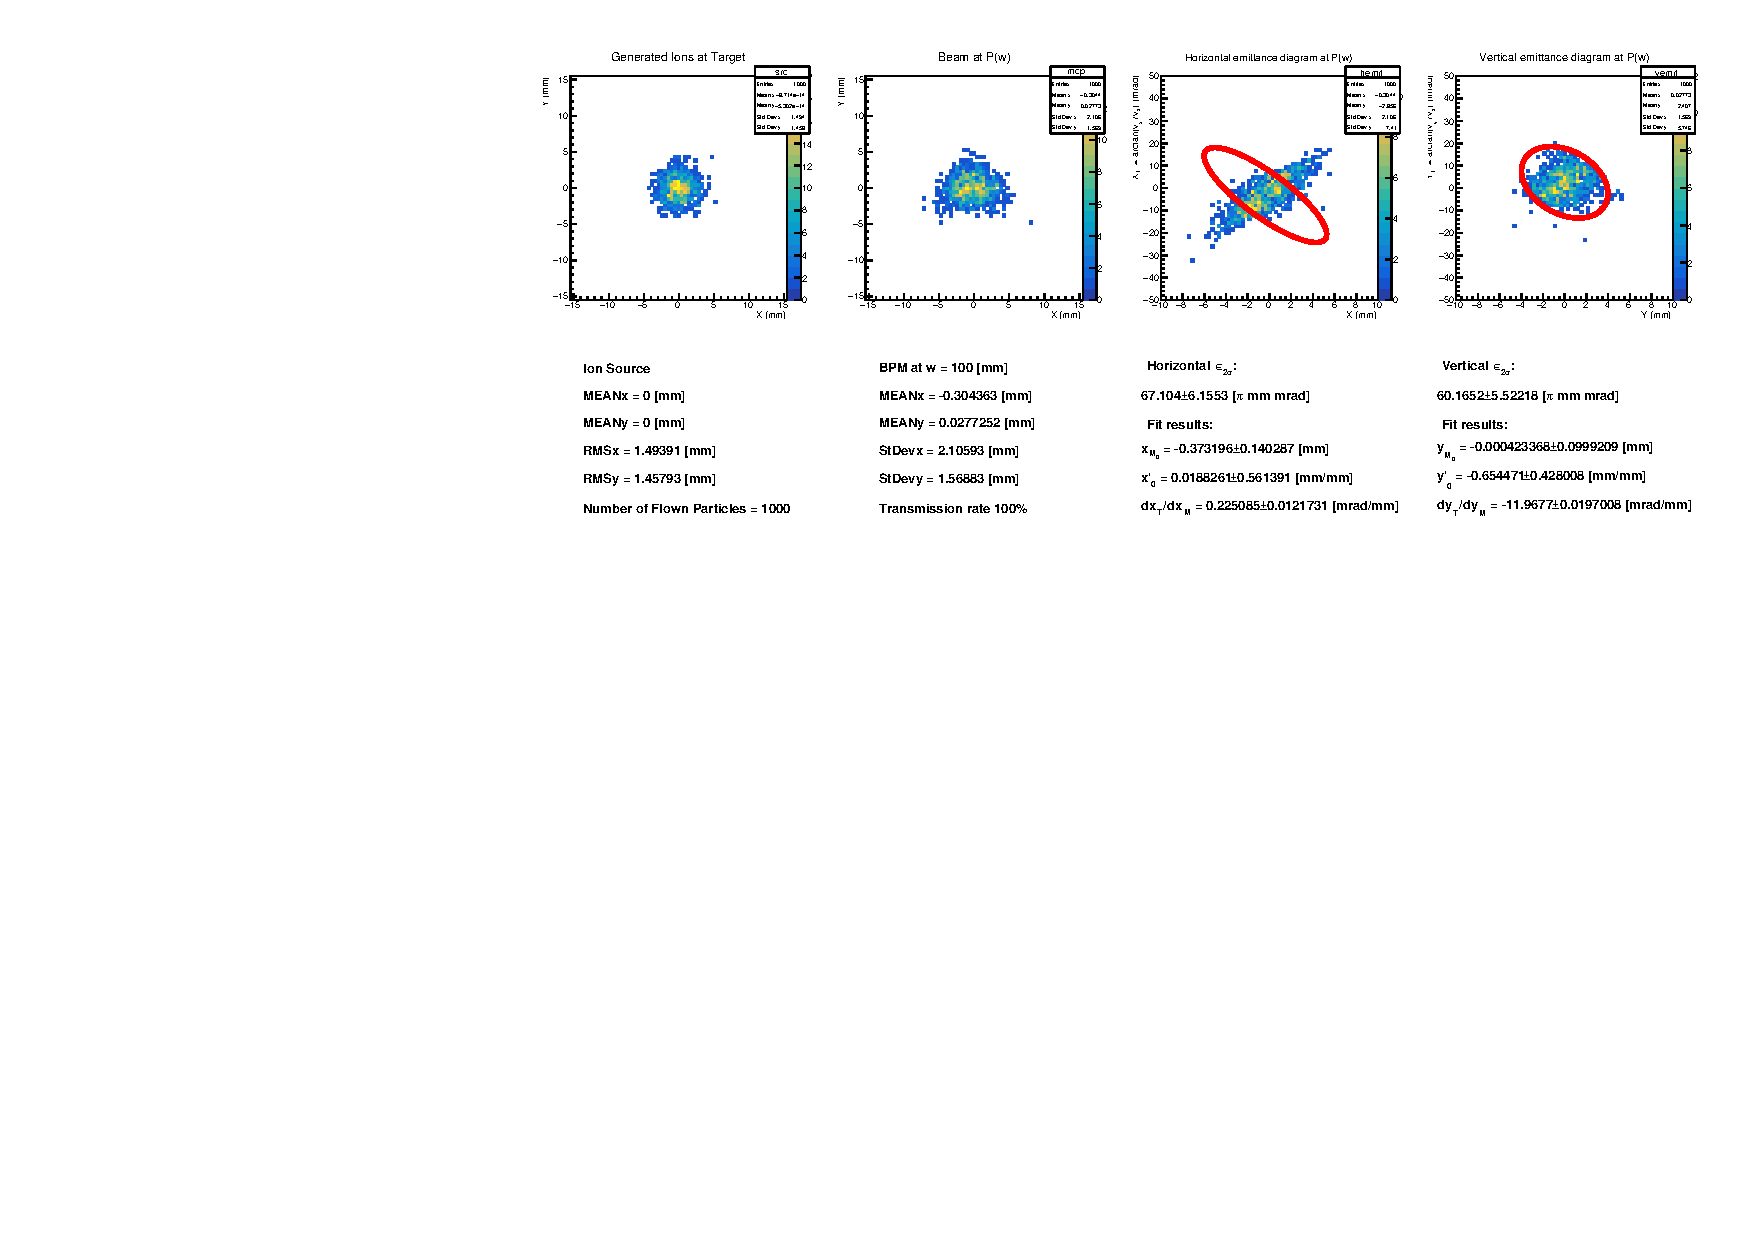
\includegraphics[clip,width=8.0cm,angle=-90]{./stdevemittance_files/emittance45_fitmethod.pdf}
    \caption{Emittance plot using the 2D fit method.\label{fig:emittancefit}}
  \end{center}
\end{figure}

\begin{figure}[H]
  \begin{center}
    \includegraphics[clip,width=8.0cm,angle=-90]{./stdevemittance_files/emittance45_statmethod.pdf}
    \caption{Emittance plot using the direct calculation method.\label{fig:emittancestat}}
  \end{center}
\end{figure}





\end{document}
